\section{Results}
\label{sec:results} 

Our visualization storyline include four parts, features, best split, feature ranking and tree model. 

\subsection{Vis 1: Features}

In this part, as shown in Figure \ref{fig:vis_1}, we selected four typical features related to users' rating, including 1) restaurant type, visualized with a bar chart, 2) restaurant location, visualized with a map, 3) frequent words related to different ratings, visualized with a word cloud, 4) friendship network, visualized with a network. With these four selected features and different visualizations, we aimed to illustrate the difference of features. In each visualization, we added the rating information by either using the tooltip or other methods to show how the features are related to user's rating. 

%-------------------------------------------
\begin{figure}[h]
	\centering
	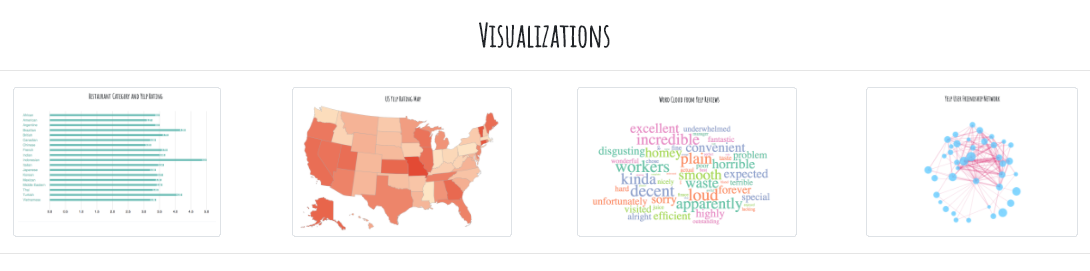
\includegraphics[width=9cm]{vis_1.png}
	\caption{Visualizations of selected features related to users' rating.}
	\label{fig:vis_1}
\end{figure}
%------------------------------------------- 

\subsection{Vis 2: Best Split}

As to demonstrate how different cut-offs would influence the prediction results, we used user's average rating as an example, to illustrate the influence of thresholds on correct and other rates in the prediction results. The best split is determined by choosing the right threshold of the feature. As shown in Figure \ref{fig:vis_2}, when the threshold of user average rating is changed, the correct, incorrect, true positive, positive rate would all change. For all the features used for rating prediction, their best splits would be determined in advance. 

%-------------------------------------------
\begin{figure}[h]
	\centering
	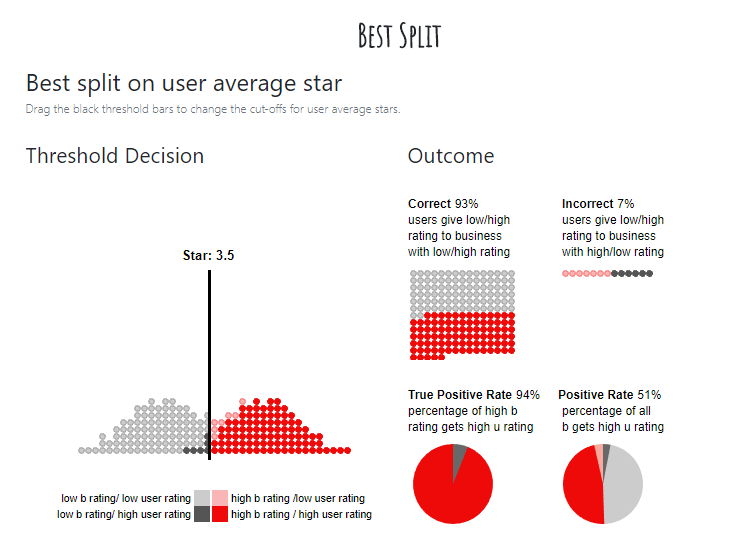
\includegraphics[width=9cm]{vis_2.png}
	\caption{Visualizations of how to choose best split.}
	\label{fig:vis_2}
\end{figure}
%------------------------------------------- 

\subsection{Vis 3: Feature Ranking}

As shown in Figure \ref{fig:vis_3}, with the feature ranking results shown in Table \ref{tb:ranking}, we further visualize the result using an radar map. This map illustrate the importance of different features in rating prediction. This is an important process before generating the tree model as only high ranked features would be used in the tree model. 

%-------------------------------------------
\begin{figure}[h]
	\centering
	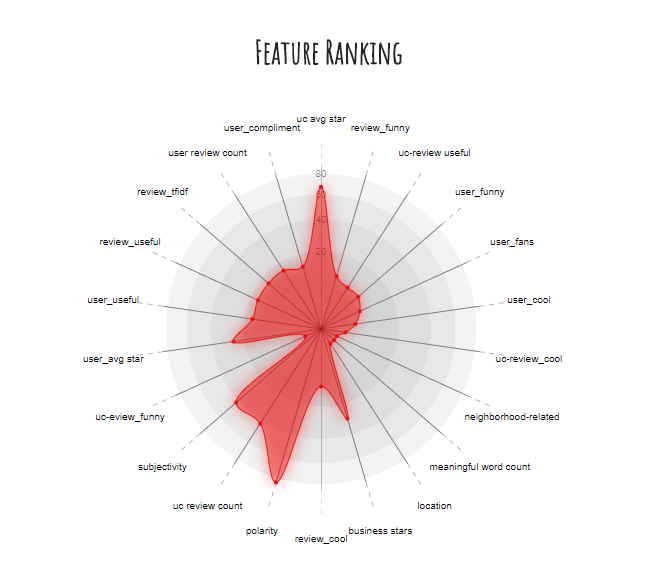
\includegraphics[width=9cm]{vis_3.png}
	\caption{Visualizations of feature ranking result.}
	\label{fig:vis_3}
\end{figure}
%------------------------------------------- 

\subsection{Vis 4: Tree Model}

Finally, with selected features from ranking, we built the decision tree model for rating prediction as shown in Figure \ref{fig:vis_4}. This visualization include the basic tree model with nodes represent the class labels and edges represent conjunctions of feature that lead to the class labels. This tree map works in a dynamic way of showing how a given input would be classified, i.e., how a user's rating would be predicted given related features. Additionally, the training and test accuracy are also calculated. 

%-------------------------------------------
\begin{figure}[h]
	\centering
	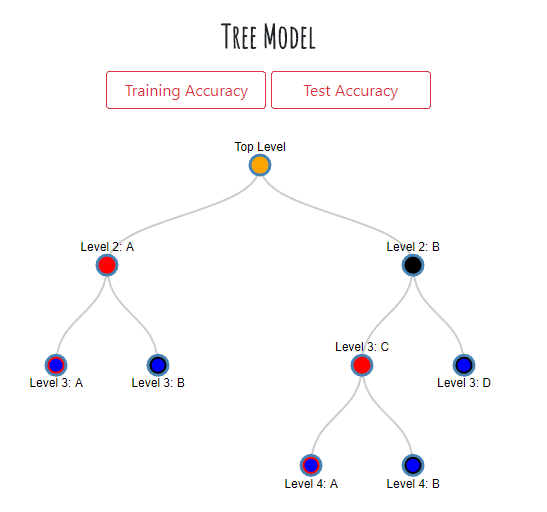
\includegraphics[width=9cm]{vis_4.png}
	\caption{Visualizations of tree model and training/test accuracy.}
	\label{fig:vis_4}
\end{figure}
%-------------------------------------------
